%chapter 1

\chapter{Literature Review} % Write in your own chapter title
\label{Chapter1}
\lhead{Chapter 1. \emph{Literature Review}} % Write in your own chapter title to set the page header

\section{Introduction}
\section{Rectifier}
Unlike diode rectifiers, PCRs or phase controlled rectifiers
has an advantage of regulating the output voltage. The diode
rectifiers are termed as uncontrolled rectifiers. When 
these diodes are switched with Thyristors, then it becomes 
phase control rectifier. The o/p voltage can be regulated 
by changing the firing angle of the Thyristors. The main 
application of these rectifiers is involved in speed control 
of DC motor.
\subsection{Phase Controlled Rectifier}
The term PCR or Phase controlled rectifier is a one type of 
rectifier circuit in which the diodes are switched by Thyristors 
or SCRs (Silicon Controlled Rectifiers). Whereas the diodes offer
no control over the o/p voltage, the Thyristors can be used 
to differ the output voltage by adjusting the firing angle or 
delay. A phase control Thyristor is activated by applying a short 
pulse to its gate terminal and it is deactivated due to line 
communication or natural. In case of heavy inductive load, it is 
deactivated by firing another Thyristor of the rectifier during 
the negative half cycle of i/p voltage.

\subsection{Three-phase bridge rectifier controlled}
The controlled three-phase bridge rectifier uses thyristors in 
place of diodes. The output voltage is reduced by the factor cos(a).

\begin{equation}
	V_{dc}=\frac{3\sqrt{3}V_{peak} cos{\alpha} }{\pi}
\end{equation}
Or, expressed in terms of the line to line input voltage:
\begin{equation}
	V_{dc}=\frac{3V_{LLpeak} cos{\alpha} }{\pi}
\end{equation}

Where:
\\VLLpeak, the peak value of the line to line input voltages.
\\Vpeak, the peak value of the phase (line to neutral) input voltages.
\\a, firing angle of the thyristor (0 if diodes are used to perform rectification).
The above equations are only valid when no current is drawn from the AC 
supply or in the theoretical case when the AC supply connections have no inductance.
In practice, the supply inductance causes a reduction of DC output voltage 
with increasing load, typically in the range 10–20 \% at full load.

The effect of supply inductance is to slow down the transfer process 
(called commutation) from one phase to the next. As result of this is 
that at each transition between a pair of devices, there is a period 
of overlap during which three (rather than two) devices in the bridge 
are conducting simultaneously. The overlap angle is usually referred 
to by the symbol mu (or u), and may be 20 30° at full load.\\
With supply inductance taken into account, the output voltage of the
rectifier is reduced to.
\begin{equation}
	V_{dc}=\frac{3V_{LLpeak} cos{\alpha} }{\pi}
\end{equation}
\begin{figure}[htbp]
	\centering
		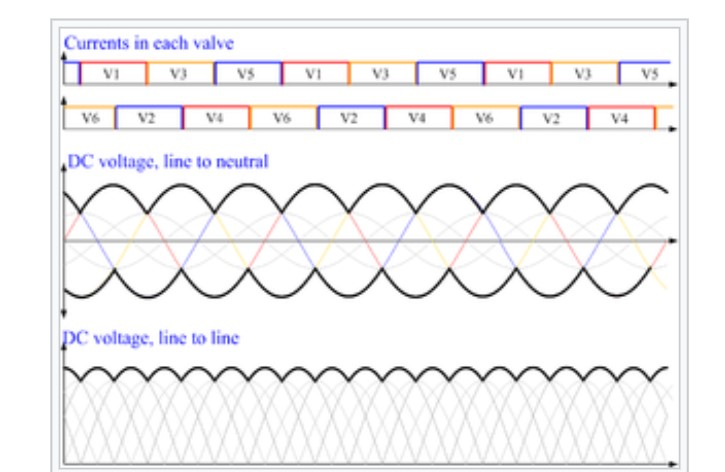
\includegraphics[width = 4in]{./Figures/rectifier.jpg}
		\rule{35em}{5pt}
	\caption{Outputs of Rectifier for firing agle zero}
	\label{fig:1}
\end{figure}
\newpage 
\section{Inverter}
A power inverter, or inverter, is an electronic device that converts direct current (DC) to alternating current (AC).
The input voltage, output voltage and frequency, and overall power handling depend on the design of the specific circuitry[1].\\ 
Inverters can be divided into two kinds:
\begin{itemize}
\item Voltage Source Inverters (VSI)
\item Current Source Inverters (CSI)
\end{itemize}
\begin{figure}[htbp]
	\centering
		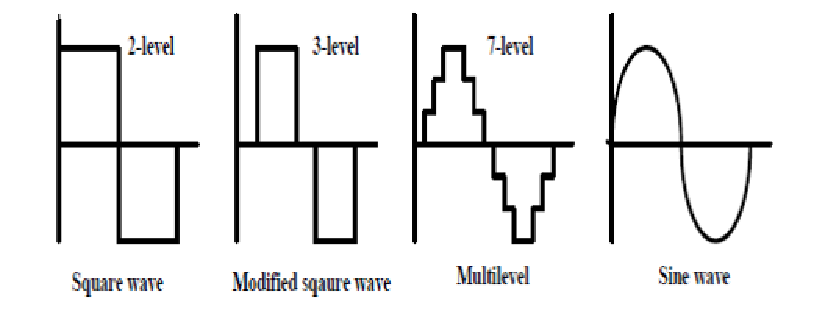
\includegraphics[width = 4in]{./Figures/Picture1.pdf}
		\rule{35em}{5pt}
	\caption{Outputs of Inverters at Zero firing angle}
	\label{fig:1}
\end{figure}
The basic component of an inverter is fast working switch like
IGBT or MOSFET.However, later is more preferred because main 
advantage of a MOSFET is that it requires almost no input current 
to control the load current, when compared with IGBT.
\subsection{MOSFET}
The MOSFET [\ref{fig:2}] is a type of field-effect transistor (FET), most commonly fabricated by the controlled oxidation of silicon. It has an insulated gate, whose voltage determines the conductivity of the device. This ability to change conductivity with the amount of applied voltage can be used for amplifying or switching electronic signals.\\
The Mosfet is further divided into n-channel Mosfet and p-channel Mosfet depending upon formation and has three modes of opertion as :
\begin{itemize}
\item Cutoff mode
\item Ohmic mode
\item Active mode
\end{itemize}
For switciing purposes Mosfet is used in active and cutoff mode.
  \begin{figure}[htbp]
	\centering
		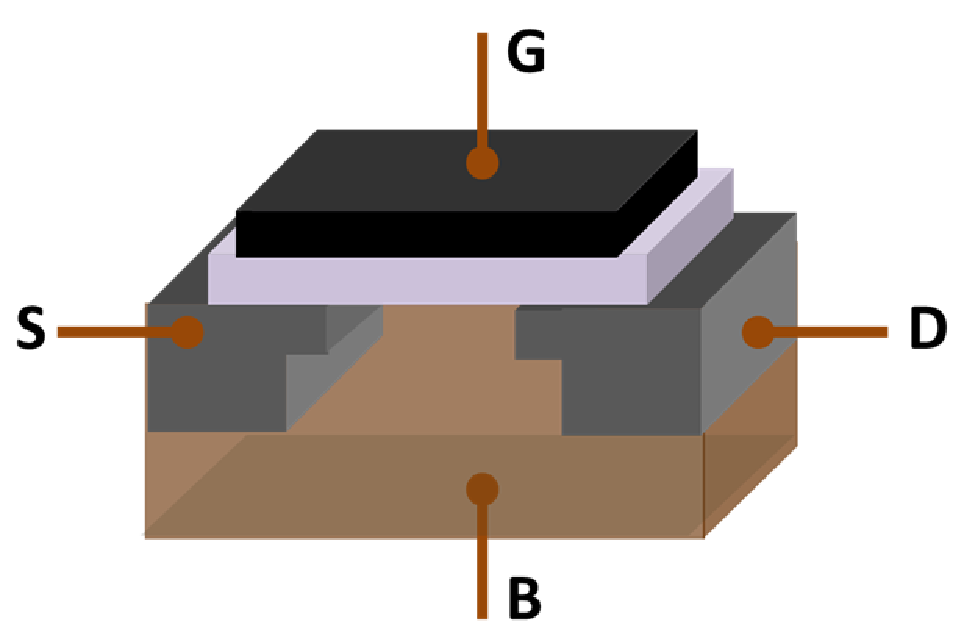
\includegraphics[width = 2in]{./Figures/Mosfet.pdf}
		\rule{35em}{5pt}
	\caption{ MOSFET showing gate (G), body (B), source (S) and drain (D) terminals. The gate is separated from the body by an insulating layer (white)}
	\label{fig:2}
\end{figure}
\section{Hierarchy of Inverter}
General Hierarchy of inverter\ref{fig:3} is shown below.Under the perspective of project the selective hierarchy will start from basic inverter to unequal dc sources cascaded h-bridge multilevel inverters.   
\begin{figure}[htbp]
	\centering
		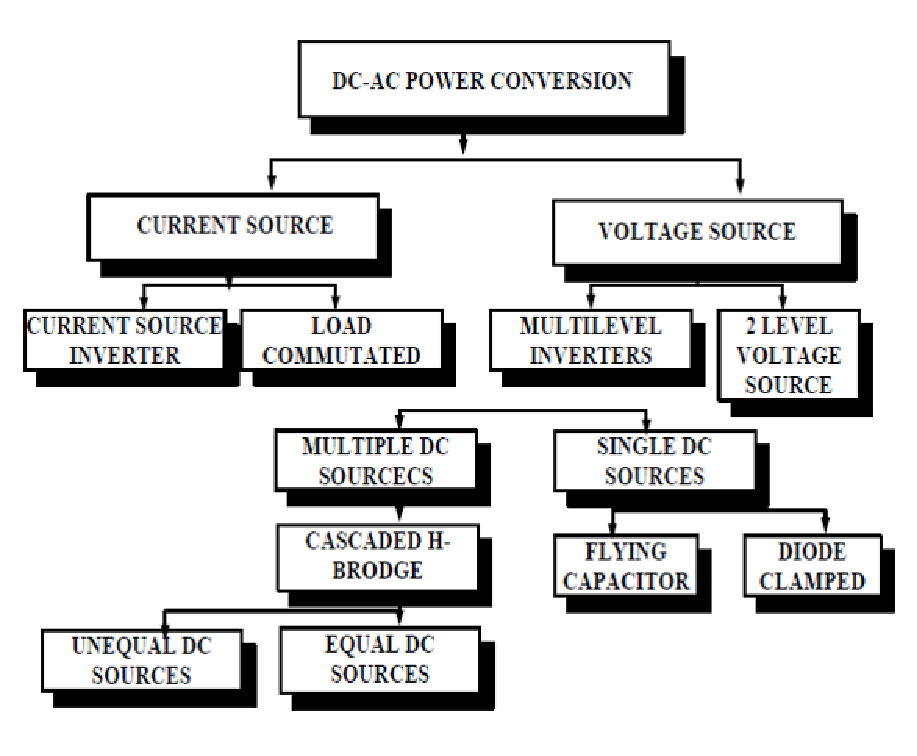
\includegraphics[width = 3in]{./Figures/Picture2.pdf}
		\rule{35em}{5pt}
	\caption{Hierarchy of inverter}
	\label{fig:3}
\end{figure}
\section{Voltage Source Inverter}
 If the input dc is voltage source, the inverter is called a voltage
source inverter.The VSI circuit has direct control over output (ac)
voltage. Shape of voltage wave-forms output by an ideal VSI should be independent of load connected at the output.\\
The simplest dc voltage source for a VSI may be a battery bank, which may consist of several cells in series-parallel combination.A voltage source is called stiff, if the source voltage magnitude does not depend on load connected to it. All VSI assume stiff voltage supply at the input.Some examples where voltage source inverters are used are: UPS units, adjustable speed drives (Automatic Star Delta) for ac motors, electronic frequency changer circuits etc.\\
The achievable magnitude of ac voltage is limited by the magnitude of inputc dc voltage. In some cases the inverter output voltage is stepped up using a transformer to meet the load requirement. 
VSI is further divided into two types:
\begin{itemize}
\item Multilevel Inverters
\item 2 Level Voltage Source
\end{itemize}
\section{Multilevel Inverters}
A multilevel inverter is a PE device which is capable of providing desired alternating voltage level at the output using multiple lower level DC voltages as an input.Multilevel inverters also enables the use of low power application in renewable energy sources.
These converters are suitable in high voltage and high power
applications due to:
\begin{itemize}
\item Their ability to synthesize higher voltages with a
limited maximum device rating
\item Less harmonic distortion
\item Producing of smaller common-mode voltage
\item Less electromagnetic compatibility problems
\item Attain higher voltage with a limited maximum device rating.
\end{itemize}
The range of the output power is a very important and evident
limitation of two-level inverter. However, this problem can be
overcome by introducing the concept of multilevel inverters.\\
The three most popular multilevel inverters are:
\begin{itemize}
\item Diode-Clamped Multilevel Inverter (DC-MLI)
\item Flying-Capacitor Multilevel Inverter (FC-MLI)
\item Cascaded H-Bridge Multilevel Inverter (CHBMLI)
\end{itemize}
First two use single voltage source for working while CHBMLI use multiple voltage sources.
\begin{figure}[htbp]
	\centering
		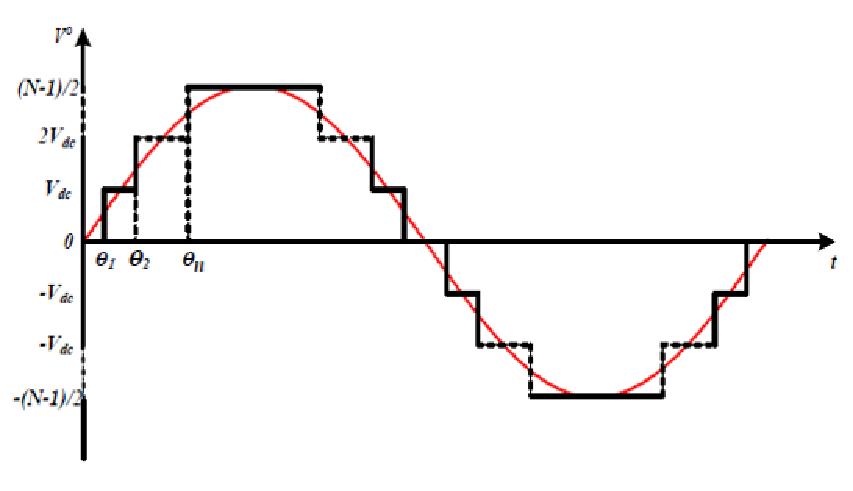
\includegraphics[width = 5in]{./Figures/Picture3.pdf}
		\rule{35em}{5pt}
	\caption{Generalized stepped waveform of multilevel inverters }
	\label{fig:4}
\end{figure}
 
\section{H Bridge}An H bridge \ref{fig:4} enables a reverse voltage to be applied across a load.\\
These circuits are often used in multiple applications to allow bidirectional movement of DC motors,
DC-to-AC converters,AC/AC converters,DC-to-DC $push–pull$ converter and many other kinds of power electronics use H bridges.\\
 An H bridge is built with four switches \ref{fig:2}. When the switches S1 and S4 are closed (and S2 and S3 are open) a positive voltage will be applied across the motor and vice versa. The point to ponder is that switches S1 and S2 should never be closed at the same time, as this would cause a short circuit on the input voltage source as seen from the figure. The same applies to the switches S3 and S4.\\
 Thus, functioning of a single H-bridge is similar to that of
conventional 2-level inverter. Each H-bridge requires an
isolated dc source/capacitor to generate its corresponding
output. The switches are activated in such a way that the
output voltage across the load terminals is the aggregation
of the voltage generated by the H-bridge.
 
\begin{figure}[htbp]
	\centering
		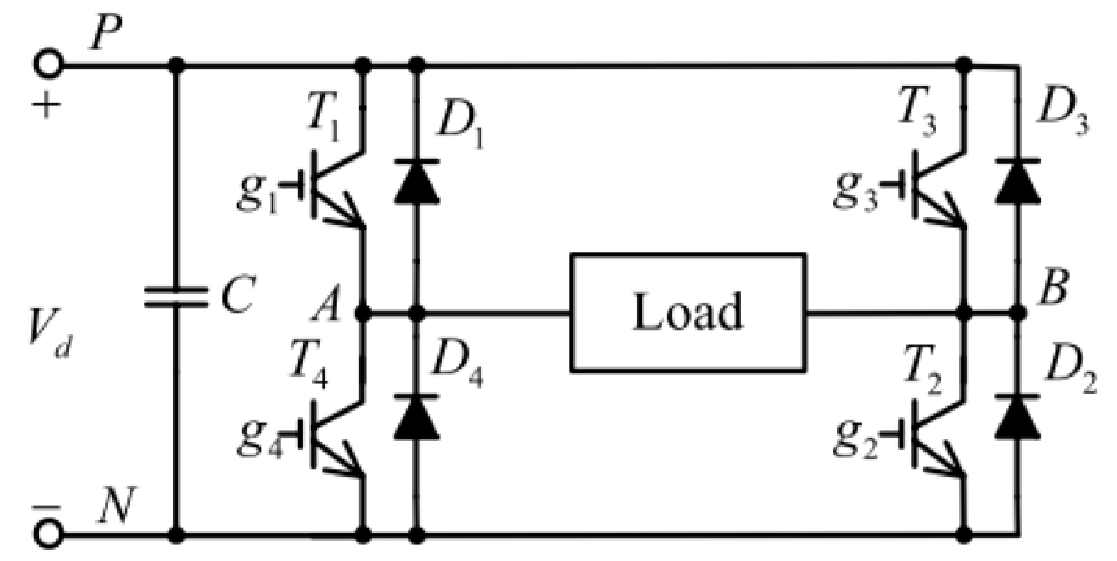
\includegraphics[width = 5in]{./Figures/h-bridge.pdf}
		\rule{35em}{3pt}
	\caption{Unit H Bridge}
	\label{fig:5}
\end{figure}
\section{Modulation Techniques for Inverter}
 The inverter dc voltage input $V_d$ is usually fixed while its ac output voltage $V_(AB)$ can be adjusted by different modulation schemes.
Main objectives of modulation strategy are as follows:
\begin{itemize}
\item Capable of operating wide range of modulation index, preferably
from 0 to 1
\item Less switching loss with improved overall efficiency
\item Less THD in output voltage
\item Obtaining high magnitude of the output fundamental frequency
component
\item Easy for implementation for practical applications
\item Less computational burden and time
\end{itemize}
However, for the inverters used in high power applications,
THD, switching losses, switching capabilities and inverter
efficiency are the critical issues that must be taken into account in
performance evaluation.
\section{Classification of Modulation Techniques}
Based on switching frequency for computational work modulation techniques are classified as follows:
\begin{itemize}
\item Sinusoidal PWM and Space Vector PWM techniques for high switching frequency.
\item Selective Harmonic Elimination and Space Vector Control for fundamental switching frequency
\end{itemize}
\begin{figure}[htbp]
	\centering
		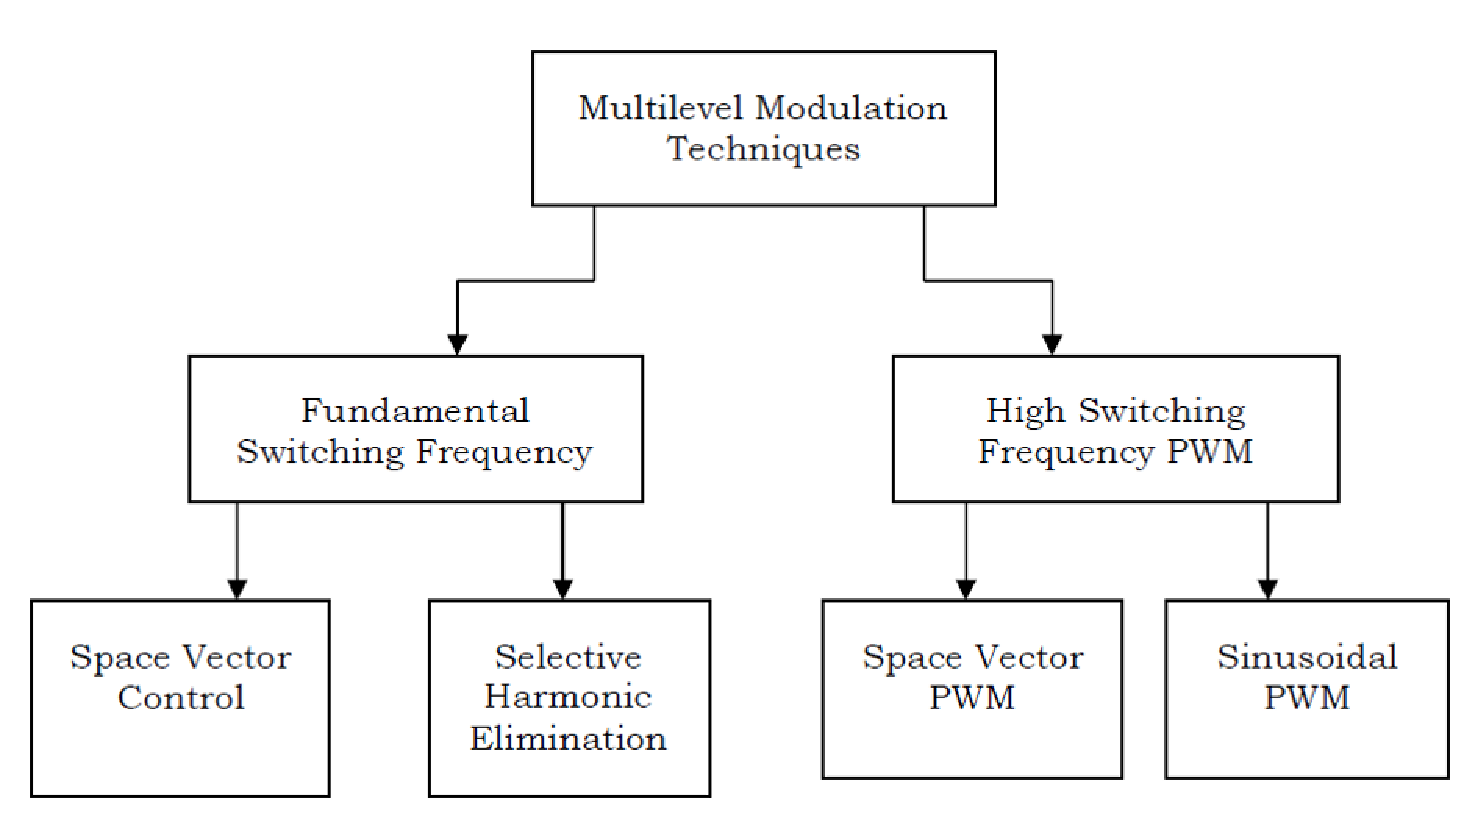
\includegraphics[width = 3.5in]{./Figures/Doc1.pdf}
		\rule{35em}{5pt}
	\caption{Classification of Modulation Techniques}
	\label{fig:9}
\end{figure}
\section{Sinusoidal PWM}
Carrier based sinusoidal PWM techniques which are employed in control CHBMLI can be
generally classified into two categories:
\begin{itemize}
\item Phase-shifted carrier based pulse width modulation technique.
\item Level-shifted carrier based pulse width modulation technique.
\end{itemize}
\subsection{Level-shifted carrier based PWM (LSCPWM) technique}
Level-shifted carrier based PWM (LSCPWM) technique is used to control neutral point clamped inverter and to control cascaded multilevel inverters. This technique has drawbacks such as uneven distribution of power among cells and high THD in output voltage and current wave forms.
LSCPWM is further divided into three categories:
\begin{itemize}
\item Phase Disposition (PD-PWM):
 wherein all the carrier signals are in same phase.
\item Phase Opposition Disposition (POD-PWM):
wherein the carrier signals above the zero are out of phase with those below the zero by $180^o$.
\item Alternative Phase Opposition Disposition (APOD-PWM):
 wherein the adjacent carrier signals are out of phase by $180^o$.
\end{itemize}
\subsection{Phase shifted carrier based PWM (PSCPWM) technique}
 Phase shifted carrier based pulse width modulation
(PSCPWM) technique is commonly used modulation technique for
control of cascaded multilevel inverters because of the following
reasons:
\begin{itemize}
\item Better harmonic profile of output voltage and current
wave-forms.
\item Even power distribution among levels.
\item Easy to implement independently. 
\end{itemize}
These advantages made PSCPWM technique popular compared to LSCPWM technique to control CHB multilevel inverters.\\
Generally, a multilevel inverter with m-level voltage requires $m-1$ triangular carriers. All the carriers have same frequency and same peak-to-peak amplitude with phase shift($\phi_(cr)$ )between adjacent carrier waves  and is given by
$$\phi_(cr)=\frac{360^o}{m-1} $$

The modulating signal is usually a three-phase sinusoidal wave
with adjustable amplitude and frequency. By comparing the
modulated wave $V_(mA)$ with the carrier waves gate signals are
generated.
 The fundamental voltage component in the inverter output
voltage can be controlled by modulation index $M_I$. Modulation index
is the ratio of maximum voltage value of modulating wave $V_m$ to
carrier wave voltage $V_(cr)$.
The modulation index $M_I$ is usually adjusted by varying $V_m$ by
keeping $V_(cr)$ fixed.
$$M_I=\frac{V_m}{V_(cr)}$$
Harmonics in the case the of high switching
frequency modulation techniques appears as side-bands around
carrier frequency produces high THD which results in trouble some
filtering.For the project case multi-carrier sinusoidal PWM technique is used.
\section{LCL filter}
The use of a LCL-filter mitigates the switching ripple injected in the grid by a three-phase
active rectifier or Three-phase inverter (VSI). However stability problems could arise in the
current control loop. In order to overcome them a damping resistor can be inserted, at the cost of
efficiency. On the contrary the use of the active damping seems really attractive but it is often
limited by the use of more sensors with respect to the standard control and by the complex tuning
procedure.
\begin{figure}[htbp]
	\centering
		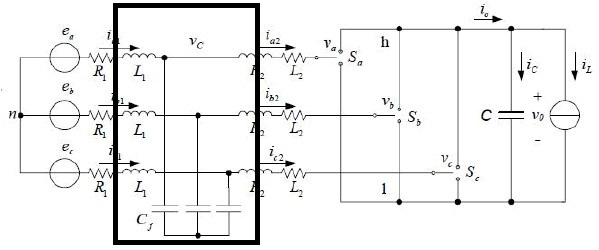
\includegraphics[width = 4in]{./Figures/LCLfilter.jpg}
		\rule{35em}{5pt}
	\caption{LCLfilter Circuit}
	\label{fig:1}
\end{figure}